\chapter{Metodología}
\label{ch:metodologia}

\quad En este apartado se empezará explicando los programas que se han utilizado y el proceso de creación del modelo.


\section{Software utilizado}

Los programas que se han utilizado para la realización de este \gls{pfg} son:

\subsection{draw.io}

Todos los gráficos que se han realizado han sido hechos utilizando la herramienta online \href{https://www.draw.io}{draw.io}. 

\textit{Draw.io} es una herramienta online capaz de crear diagramas de flujo, organigramas, \textit{wireframes}, diagramas en UML y diagramas de redes. Está hecha en HTML 5 y JavaScript\cite{drawio}.

\begin{figure}[H]
	\centering
	
\includegraphics[width=0.2\textwidth]{figures/drawio.png}
	\caption{\label{fig:drawio}Logotipo de drawio. Fuente: \cite{drawio}}
\end{figure}

\subsection{Python}

Python es un lenguaje de programación interpretado de alto nivel. Se distingue por ser multiparadigma, lo que significa que ofrece soporte parcial para la orientación a objetos, la programación imperativa y, en menor medida, la programación funcional\cite{python}.

\begin{figure}[H]
	\centering
	
\includegraphics[width=0.2\textwidth]{figures/pythonlogo.png}
	\caption{\label{fig:python}Logotipo de Anaconda. Fuente: \cite{python}}
\end{figure}

Python permite el uso de paquetes los cuales se pueden instalar. Los paquetes que se han utilizado son:

\begin{itemize}
	\item \textbf{Tensorflow con Keras}: Tensorflow es una biblioteca de código abierto creada por Google para aprendizaje automático\cite{wiki_tensorflow,tensorflow_website}. Keras también es una biiblioteca de código abierto la cual se puede ejecutar sobre Tensorflow para crear redes de neuronas\cite{keras_website}.
	\item \textbf{Numpy}: Numpy es una biblioteca que se utiliza para manejar vectores y matrices\cite{numpy}.
	\item \textbf{Os}: OS es una biblioteca por defecto para llamar operaciones del sistema operativo.
	\item \textbf{Pillow}: Pillow es una biblioteca que sirve para cargar, guardar y mostrar imágenes por pantalla.
	\item \textbf{Matplotlib}: Matplotlib es una biblioteca que se utiliza para mostrar gráficas.
	\item \textbf{Time}: Time se utiliza para llamar conseguir valores como la hora o la fecha del sistema operativo.
	\item \textbf{IPython}: Es un \textit{shell} interactivo de Jupyter Notebooks que añade más funcionalidades.
	\item \textbf{Pandas}: Pandas es una biblioteca que se utiliza para crear, cargar y guardar conjuntos de datos llamados Datasets.
\end{itemize}

Laversión utilizada de python es la \textbf{3.9.18}.

\subsection{Anaconda}

Anaconda es un programa de código abierto que sirve para simplificar la gestión de paquetes en Python y R\cite{anacondaWiki}.

\begin{figure}[H]
	\centering
	
\includegraphics[width=0.3\textwidth]{figures/anaconda_logo.jpg}
	\caption{\label{fig:anaconda}Logotipo de Anaconda. Fuente: \cite{anacondaRTD}}
\end{figure}

En este \gls{pfg} se ha utilizado para facilitar la instalación de tensorflow y cuda para poder entrenar las redes de neuronas en local con una \gls{gpu}.

\subsection{Visual Studio Code}

Visual studio code es un editor de código fuente de código abierto creado por \textit{Microsoft}. Este editor permita la instalación de extensiones que permiten manejar diferentes lenguajes de programación.

\begin{figure}[H]
	\centering
	
\includegraphics[width=0.3\textwidth]{figures/vsc.png}
	\caption{\label{fig:vscodeicon}Logotipo de Visual Studio Code. Fuente: \cite{vscodeicon}}
\end{figure}

\subsection{Extensión de visual Studio Code: Jupyter Notebooks}

Jupyter es una organización sin ánimo de lucro que alberga una variedad de productos diseñados para la computación interactiva y la colaboración en ciencia de datos y computación científica. Uno de sus productos más destacados es Jupyter Notebook, un entorno interactivo basado en la web que permite la creación de documentos en los que se puede combinar código ejecutable, texto enriquecido, visualizaciones y otros elementos multimedia.

\begin{figure}[H]
	\centering
	
\includegraphics[width=0.2\textwidth]{figures/jupyterlogo.jpg}
	\caption{\label{fig:jupyterlogo}Logotipo de Jupyter. Fuente: \cite{jupyter_wikipedia}}
\end{figure}

La extensión de Jupyter para Visual Studio Code ha sido creada por \textit{Microsoft} y permite la creación de estos notebooks en la propia plataforma.

\subsection{Microsoft Excel}

Microsoft excel es un program desarrollado por Microsoft para visualizar, cargar guardar y editar hojas de cálculo\cite{excel_microsoft}.

\begin{figure}[H]
	\centering
	
\includegraphics[width=0.2\textwidth]{figures/excellogo.png}
	\caption{\label{fig:excellogo}Logotipo de Jupyter. Fuente: \cite{excel_wikipedia}}
\end{figure}


\section{Creación del Dataset}

\quad Se ha utilizado el dataset DIV2K. El dataset DIV2K fue creado en 2017 por un equipo de investigadores de la Universidad Técnica de Múnich y de la Universidad de Ciencia y Tecnología de Pohang, Corea del Sur \cite{Agustsson_2017_CVPR_Workshops,8014884}.

El dataset cuenta con 1,000 imágenes de alta resolución, de las cuales 800 son para entrenamiento y las 200 restantes para validación y prueba.

Antes de realizar cualquier procesamiento, se examinó la resolución de las imágenes y se decidió reescalarlas a 1024x1024x3. A las imágenes con esta resolución se les denominará de alta resolución. Esta decisión se tomó principalmente porque no todas las imágenes tienen la misma resolución y debido a las limitaciones computacionales.

\begin{figure}[H]
	\centering
	\begin{subfigure}{.4\textwidth}
		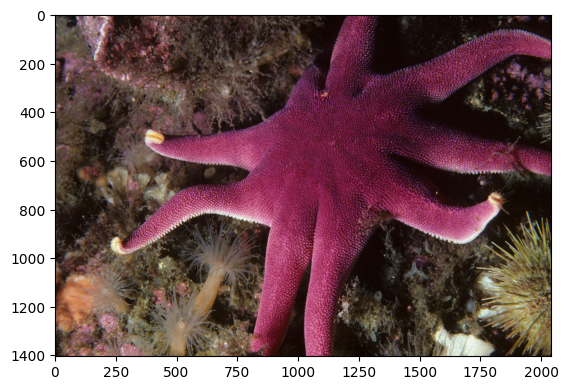
\includegraphics[width=\linewidth]{figures/div2k1.png}
		\caption{}
		\label{fig:div2k1}
	\end{subfigure}%
	\begin{subfigure}{.2\textwidth}
		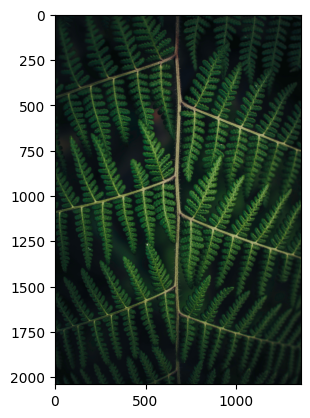
\includegraphics[width=\linewidth]{figures/div2k2.png}
		\caption{}
		\label{fig:div2k2}
	\end{subfigure}%
	\caption{Comparación de imágenes en el dataset DIV2K Fuente:\cite{Agustsson_2017_CVPR_Workshops,8014884}}
	\label{fig:div2k}
\end{figure}

Se han creado 3 datasets diferentes dependiendo del escalado de la imagen:

\begin{itemize}
	\item \textbf{Dataset escala x1 (De 1024x1024 a 1024x1024)}: Este dataset contiene pares de imágenes de alta resolución con la misma resolución, es decir,dos imágenes de 1024x1024x3.
	\item \textbf{Dataset escala x2 (De 512x512 a 1024x1024)}: Este dataset contiene pares de imágenes con distinta resolución, una con resolución media, es decir, 512x512x3, y la otra con resolución alta.
	\item \textbf{Dataset escala x4 (De 256x256 a 1024x1024)}: Este dataset contiene también pares de imágenes con distinta resolución, una con baja resolución, es decir, 256x256x3, y la otra con alta resolución.
\end{itemize}


En cada dataset, se han cogido las imágenes de alta, media y baja resolución y se les a aplicado una transformación siguiendo el criterio de \cite{Wavelet,OWLNet} con la fórmula \ref{eq:detfunc} mencionada en el apartado \ref{ch:estado del arte}. Es decir, se les ha aplicado una función de \textbf{desenfoque} a la imagen y ese resultado se le a añadido \textbf{ruido}.

La función de desenfoque, obtenida de \cite{blzq2023gist},es la siguiente:

\begin{lstlisting}[language=python]
	def gaussian_blur(img, kernel_size=2, sigma=50):
		def gauss_kernel(channels, kernel_size, sigma):
			ax = tf.range(-kernel_size//2+1.0,kernel_size//2+1.0)
			xx, yy = tf.meshgrid(ax, ax)
			kernel = tf.exp(-(xx ** 2 + yy ** 2)/(2.0 * sigma ** 2))
			kernel = kernel / tf.reduce_sum(kernel)
			kernel = tf.tile(kernel[...,tf.newaxis],[1, 1,channels])
			return kernel
	gaussian_kernel = gauss_kernel(tf.shape(img)[-1],kernel_size,sigma)
	gaussian_kernel = gaussian_kernel[..., tf.newaxis]
	img = tf.expand_dims(img, axis=0)  
	img_blurred = tf.nn.depthwise_conv2d(img, gaussian_kernel,
						[1, 1, 1, 1], padding='SAME', data_format='NHWC')
	img_blurred = tf.squeeze(img_blurred, axis=0)  
	return img_blurred
\end{lstlisting}

La función gaussian blur aplica un desenfoque gaussiano a una imagen utilizando TensorFlow. Primero, crea un \textit{kernel} gaussiano en función del tamaño del  \textit{kernel} y sigma. Luego, expande la dimensión de la imagen para realizar una convolución 2D con este  \textit{kernel}, aplicando el desenfoque. Finalmente, devuelve la imagen desenfocada eliminando la dimensión añadida temporalmente.

La función de ruido es la siguiente:

\begin{lstlisting}[language=python]
	
def corrupt_part_of_image(image, noise_level, corruption_level=0.04):
	mask = tf.random.uniform(tf.shape(image)[:2]) < corruption_level
	noise = tf.random.normal(tf.shape(image), stddev=noise_level)
	noise = (noise + 1.0) / 2.0
	corrupted_image = tf.where(mask[..., tf.newaxis],
				tf.clip_by_value(image + noise, 0.0, 1.0), image)
	return corrupted_image
\end{lstlisting}

Esta función realiza las siguientes operaciones: primero, crea una máscara aleatoria para determinar qué partes de la imagen serán corrompidas. Luego, genera ruido con un nivel específico y lo añade a las partes seleccionadas, asegurándose de que los valores de los píxeles permanezcan en el rango válido [0, 1]. Finalmente, devuelve la imagen con las partes afectadas por el ruido.

\begin{figure}[H]
	\centering
	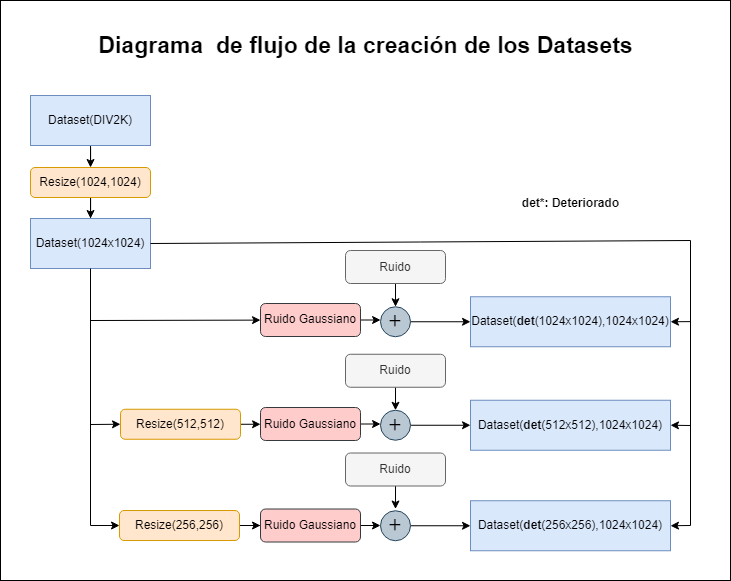
\includegraphics[width=0.9\textwidth]{figures/flow_diagram_datasets.png}
	\caption{\label{fig:datasets}Diagrama de flujo de la creación de los Datasets. Fuente: Elaboración propia}
\end{figure}

Cada dataset tiene un tamaño de lotes (o \textit{batch size}) de 1. 

Con los datasets ya listos se pasa a la siguiente fase, la creación de los modelos y su entrenamiento.

\section{Creación de Modelos y Entrenamiento}

Lo siguiente que se ha realizado es la creación y el entrenamiento de los modelos. 

Para dar más contexto del hardware utilizado en el entrenamiento de cada red de neuronas, cada red se ha entrenado de forma local en un ordenador de sobremesa con las siguientes especificaciones:

Para cada arquitectura se han creado tres modelos diferentes para cada dataset, a excepción del \gls{vae} que únicamente se ha reslizado un modelo.

\begin{itemize}
	\item CPU: Intel Core i5 de 13ª generación.
	\item RAM: 16G de memoria RAM.
	\item GPU: NVIDIA GTX 3080 de 10G de memoria.
\end{itemize}

\subsection{Autoencoder}

\subsubsection{Creación de los modelos}

\quad Se han hecho tres arquitecturas de redes de neuronas adaptado para cada dataset. El inicio de los tres autoencoders es la siguiente: se han puesto tres capas de convolución seguidas cada una de ellas con una capa de MaxPooling, luego, se han puesto otras tres capas de convolución seguidas cada una de ellas con una capa de UpSampling. A partir de aquí cada modelo es diferente:

\begin{itemize}
	\item Para el modelo de alta resolución se ha puesto una capa final de convolución.
	\item Para el modelo de media resolución se ha puesto una capa extra de convolución seguida de una capa de UpSampling, y por último, una capa de convolución.
	\item Para el modelo de baja resolución se han puesto dos capas extra de convolución seguidas cada una de ellas con una capa de UpSampling, y por último, una capa de convolución.
\end{itemize}

Todas las capas intermedias tienen la función de activación \textit{relu} y la capa final tiene la función de activación \textit{sigmoidea}.

\begin{figure}[H]
	\centering
	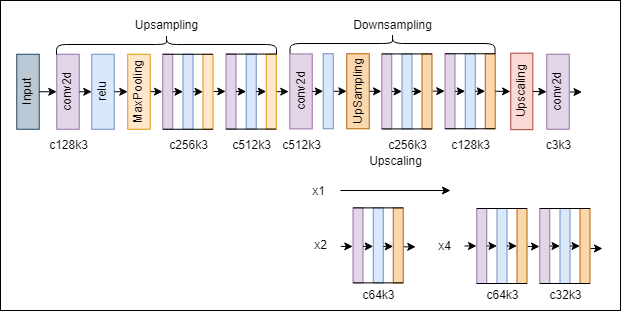
\includegraphics[width=1\textwidth]{figures/autoencoder.png}
	\caption{\label{fig:autoencoder}Composición del autoencoder. Los valores debajo de la convolución significan: c el número de filtros y k el tamño del kernel. Fuente: Elaboración propia}
\end{figure}

\subsubsection{Entrenamiento de los modelos}

Para el entrenamiento de este modelo se ha utilizado como función de pérdida \gls{mae} con el optimizador adam.

Para estimar la cantidad de epochs necesarios para el entrenamiento, se ha puesto un valor alto y se ha visto el epoch donde converge la función de pérdida.

\section{VAE}

\subsubsection{Creación del modelo}

\quad En el caso del \gls{vae}, debido a su arquitectura, no se ha realizado ningún escalado, solo se ha hecho un modelo en relación al escalado. La cantidad de parámetros es tan inmensa, que además, se ha decidido crear un nuevo dataset únicamente para este modelo. Este dataset contiene parches de tamaño 64x64x3, con un tamaño de lotes de 30, del dataset DIV2K. En cuanto a la creación del modelo, es un \gls{vae} convolucional.

la arquitectura del \gls{vae} se divide en dos partes: la parte del codificador y la parte del decodificador.

El codificador comienza con cuatro filtros de convolución, teniendo el tercero un tamaño de stride de 2, con lo que divide a la mitad el alto y ancho de los filtros. La capa final del codificador termina dividiéndose en dos capas densas, la capa z\_mean y la capa z\_log\_var, lo que representa la media y la logvarianza del espacio latente. Estos dos vectores se utilizan para lo que se llama \textit{reparametrization trick}. El \textit{reparametrization trick} se utiliza para poder diferenciar las variables aleatorias continuas respecto de sus parámetros. En lugar de muestrear directamente esta distribución gaussiana $(\mu,\sigma)$, se puede muestrear una distribución gaussiana estándar  $N(0,1)$, y luego transformar este muestreo mediante la siguiente fórmula:

\begin{equation}
	z = \mu + \sigma \odot \epsilon
\end{equation}

Donde $\odot$ denota la multiplicación de cada elemento por $\epsilon$, que es una distribución gaussiana estandar (ruido).

En el caso del decodificador, tiene cinco capas de convolución transpuesta, teniendo la segunda capa un tamaño de stride de 2.

Todas las capas tienen la función de activación relu, menos la última que tiene una función de activación sigmoidea.

\subsubsection{Entrenamiento del modelo}

En cuanto al entrenamiento, se ha proporcionado un tamaño de espacio latente de 200, y se ha utilizado una función de pérdida un tanto diferente.

Como ya se vio en \ref{eq:elbo}, existe una forma más útil de escribir esta fórmula y es agrupar la parte del \textit{prior} y del \textit{decodificador} convirtiéndolo en una divergencia \textit{KL(Kullback-Leibler)}

\begin{equation}
	\ln{p_\theta(x)} \le E_{z\sim q_\phi(z|x)}[\ln{p_\theta(x|z)} + \ln{p_\theta(z)} - \ln{q_\phi(z|x)}] = -KL(q_\phi(z|x)||p(z)) + E_{z\sim q_\phi(z|x)}[\ln{p_\theta(x|z)}]
\end{equation}

La divergencia \textit{KL (Kullback-Leibler)} es una medida de la diferencia entre dos distribuciones de probabilidad y se escribe así: 

\begin{equation}
	D_{kl}(P||Q)=\sum_xP(x)\log \frac {P(x)} {Q(x)}
\end{equation}

para valores continuos y discretos.

Esto es útil cuando el valor de KL es fácil de analizar siendo: 

\begin{equation}
	-KL(q_\phi(z|x)||p(z))= \frac {1}{2}(1 + \ln\sigma_\phi^2(x) - \sigma_\phi^2(x) - \mu_\phi(x)^2)
\end{equation}

Siendo este valor el valor de pérdida del modelo al que se le va a añadir el error L2 con un factor de balance \(B\) para que sea más fiel la salida. Entonces, el error del modelo será: 

\begin{equation}
	loss = B \cdot l2(x, x') + \left(\frac {1}{2}(1 + \ln\sigma_\phi^2(x) - \sigma_\phi^2(x) - \mu_\phi(x)^2)\right)
\end{equation}


\section{cGAN: Primera aproximación}

\subsubsection{Creación de los modelos}

Como ya se ha visto, en el apartado \ref{ch:estado del arte},  las redes \gls{gan} se dividen en dos modelos: el generador y el discriminador. Para la creación de todas las redes GAN se ha seguido parte del modelo propuesto en \cite{pix2pix}.

En cuanto al generador, es un tanto distinto a los generadores de las redes \gls{gan}, en este caso, se ha decidido usar una red \acrfull{cgan}, las redes \gls{cgan} se distinguen de las redes \gls{gan} principalmente por su generador, el cual es condicionado por una imagen que se llamará \textit{input}, en vez de provenir de una distribución normal Gaussiana.

Esta red comienza con un \textit{downsampling} de cuatro capas con la siguiente estructura: primero una capa de convolución, con el valor de stride a 2 y función de activación relu, y una capa de normalización de lotes. Lo siguiente es la capa de upsampling, la cual tiene la misma estructura que la de downsampling pero en vez de cuatro capas de convolución, la substituye la convolución transpuesta. Al final una capa de \textit{upscaling} la cual dependiendo de la resolución cambia:

\begin{itemize}
	\item x1: No tiene ninguna capa.
	\item x2: Tiene una capa de convolución transpuesta, con el valor de stride a 2 y función de activación relu, seguida de una capa de normalización de lotes.
	\item x4: Tiene dos capas de convolución transpuesta, con el valor de stride a 2 y función de activación relu, seguido de cada una de ellas la normalización de lotes.
\end{itemize}

Por último hay una capa de convolución transpuesta con el valor de strides a 2 y función de activación sigmoidea.

\begin{figure}[H]
	\centering
	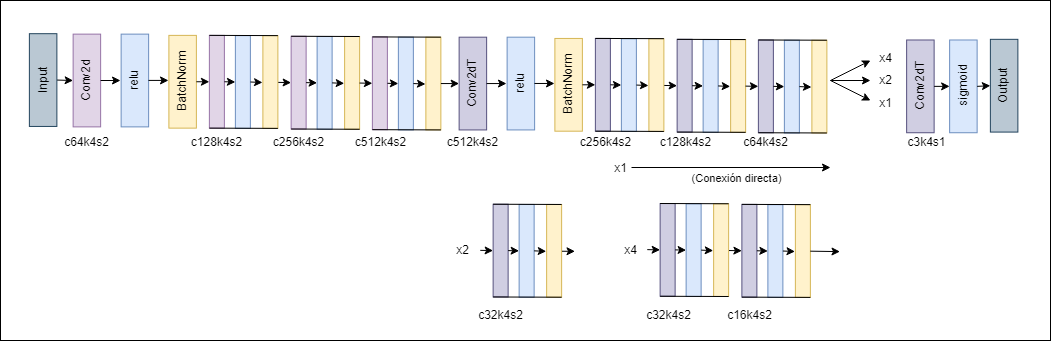
\includegraphics[width=1\textwidth]{figures/Generador_normal.png}
	\caption{\label{fig:gan}Composición del generador. Los valores debajo de cada capa de convolución significan: c el número de filtros, k el tamaño del kernel y s el tamaño del stride. Fuente: Elaboración propia}
\end{figure}


El discriminador es un discriminador por parches que sigue una estructura específica para todas las redes \gls{gan} en adelante. Comienza concatenando dos entradas del mismo tamaño. A continuación, incluye una capa de downsampling que consta de una capa de convolución seguida de una capa de \textit{LeakyReLU}.

Después, se añaden tres capas de downsampling, cada una con la misma estructura: una capa de convolución seguida de una normalización de lotes y, finalmente, una capa de \textit{LeakyReLU}. Posteriormente, se incorpora un padding de ceros y se añade otra capa de downsampling similar a las anteriores pero con el valor de stride a uno. Finalmente, se incluye otra capa de padding con más ceros, seguida de una capa de convolución con un filtro.

\begin{figure}[H]
	\centering
	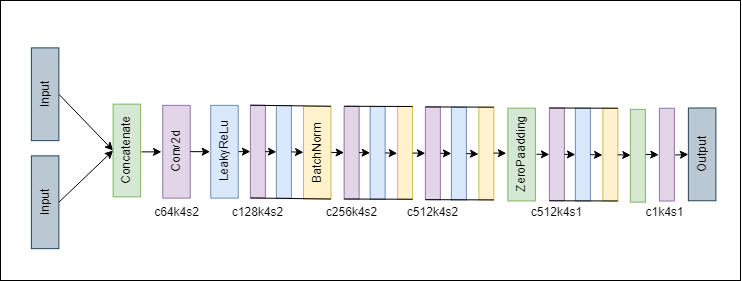
\includegraphics[width=1\textwidth]{figures/discriminator.png}
	\caption{\label{fig:discriminator}Composición del discriminador. Los valores debajo de cada capa de convolución significan: c el número de filtros, k el tamaño del kernel y s el tamaño del stride. Fuente: Elaboración propia}
\end{figure}


\subsubsection{Entrenamiento de los modelos}

Cada red tiene una función de pérdida diferente, para todos los modelos, a partir de ahora, las funciones de pérdida del generador y el discriminador van a ser las mismas.

En cuanto a la pérdida del generador, el \textit{input} se introduce tanto en el generador como en el discriminador. Antes de ingresar al discriminador, el \textit{input} se somete a un escalado bilinear para asegurar que las entradas al discriminador tengan el mismo tamaño. El generador produce una imagen que se envía al discriminador, el cual compara esta imagen generada con la imagen escalada.

El resultado del discriminador se evalúa aplicando una función de entropía cruzada sigmoidea, utilizando una matriz de unos. Además, se calcula el error absoluto medio (\gls{mae}) entre el \textit{target} y el \textit{input}, y este valor se multiplica por un factor lambda previamente definido.

Finalmente, se suman ambos errores, y el resultado se utiliza para ajustar los gradientes y actualizar el generador.


\begin{figure}[H]
	\centering
	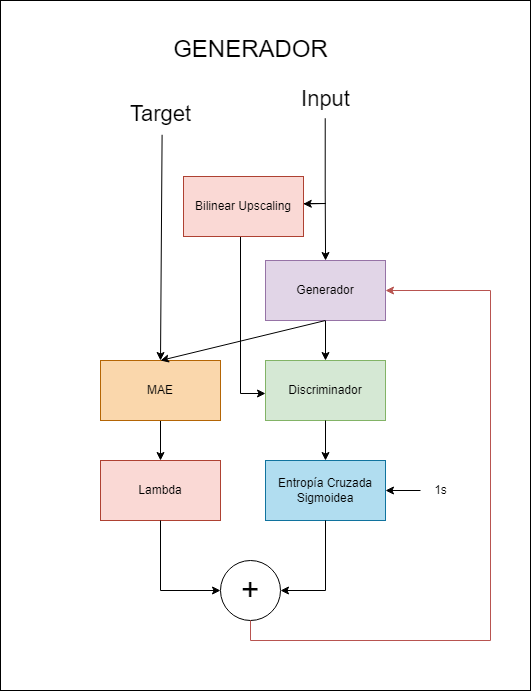
\includegraphics[width=0.5\textwidth]{figures/losses_GAN_Generador.png}
	\caption{\label{fig:gangenloss}Diagrama de flujo del cálculo del error para el generador. Fuente: Elaboración propia}
\end{figure}

En cuanto a la pérdida del discriminador, el proceso comienza con la entrada de los datos. El \textit{input} primero pasa por un escalado bilinear para que las entradas al discriminador tengan el mismo tamaño. Luego, tanto el \textit{input} escalado como el \textit{target} real se envían al discriminador.

El discriminador recibe dos conjuntos de datos: la imagen real escalada y la imagen generada por el generador. Compara estas dos imágenes para determinar la autenticidad de la imagen generada.

El resultado del discriminador se evalúa aplicando una función de entropía cruzada sigmoidea con una matriz de ceros para las imágenes generadas y una matriz de unos para las imágenes reales. Esto permite calcular la pérdida del discriminador, evaluando qué tan bien puede distinguir entre imágenes reales y generadas.

Finalmente, el error del discriminador se usa para ajustar los pesos del modelo durante el proceso de entrenamiento, mejorando su capacidad para diferenciar entre imágenes reales y generadas.

\begin{figure}[H]
	\centering
	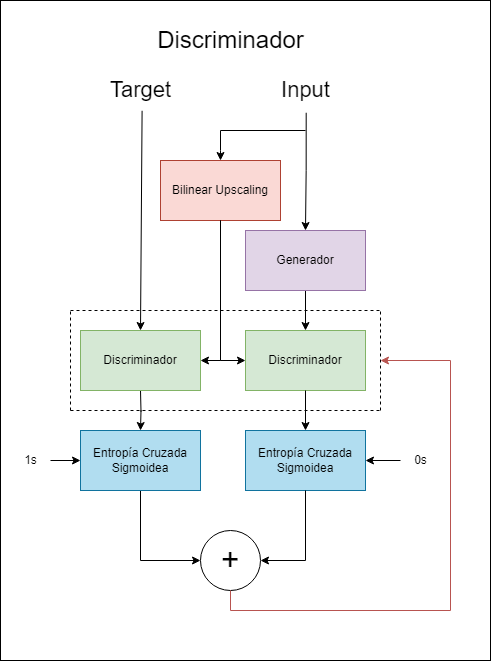
\includegraphics[width=0.5\textwidth]{figures/losses_GAN_Discriminador.png}
	\caption{\label{fig:gandiscloss}Diagrama de flujo del cálculo del error para el discriminador. Fuente: Elaboración propia}
\end{figure}


\section{cGAN: (pix2pix)}

\subsubsection{Creación de los modelos}

Este modelo fue propuesto en 2017 por....

\section{EDSR cGAN}